%!TEX root = ../thesis.tex
%\input{commands.tex}
%*******************************************************************************
%****************************** Third Chapter **********************************
%*******************************************************************************
\chapter{Haplotype phasing consistency as a signal for physical linkage in scaffolding and assembly}

% **************************** Define Graphics Path **************************
\ifpdf
    \graphicspath{{Chapter3/Figs/Raster/}{Chapter3/Figs/PDF/}{Chapter3/Figs/}}
\else
    \graphicspath{{Chapter3/Figs/Vector/}{Chapter3/Figs/}}
\fi



\section{Background}
\par{
Reference genomes have enabled a range of genomic analysis by providing prior knowledge of the sequence 
and giving genomic context as well as a common coordinate system by which to compare multiple genomes \cite{1000genomes} \cite{GRCh38}.

Assembling reference genomes is complicated by repetitive sequences, heterozygosity, and sequencing errors. As discussed in 
Chapter 3, when an assembly encounters inexact homologous sequences, it must determine which of these cases the sequence differences are due to. 
If the assembler cannot distinguish between heterozygosity and repeats, and if no reads span the homologous sequence into more unique regions, the contig must end
to avoid assembly distant regions or sequence from different chromosomes together.


Historically reference genomes were created by large haploid bacterial artificial chromosomes (BACs) clone libraries \cite{human}. 
These methods overcame much of the problem of resolving repeats and heterozygosity because of their length and the fact that they are inherently haploid. But these methods are too costly to 
apply to many genomes.
}


 More recently the cost reductions of long read technologies \cite{pacbio} \cite{oxford} 
as well as the emergence of other long range genetic information technologies \cite{10xlinked} \cite{HiC} \cite{bionano} 
have converged to make high quality, cost effective reference genomes. This has then resparked interest in assembly 
as well as large reference generation projects
such as the Earth BioGenome Project \cite{EBGP} and the Darwin Tree of Life Project.
For these technologies there are now assembly algorithms that deal with each data type \cite{falcon} \cite{supernova} \cite{bionano_assembly} 
as well as combinations of multiple technologies \cite{genemyers} \cite{hybrid10x} \cite{aedes}. 
 These methods try to co-assemble both haplotypes arriving at a haploid consensus \cite{watchtower} \cite{canu} 
 or a diploid assembly \cite{falconPHASE} \cite{supernova}, but heterozygosity injects complexity and ambiguity on top of a haploid assembly process.
 It requires that the assembler disambiguate between paralogous sequence and differences between haplotypes. When 
 the level of heterozygosity is high, the differences between haplotypes can be even greater than the differences between paralogous 
 sequences. One method for dealing with the problem of heterozygosity is inbreeding organisms to a point of low heterozygosity \cite{drosophila}, 
but this is not possible for all organisms. Trio-sga used pedigree sequencing information in the assembly algorithm \cite{trio-sga} 
but does not work on long read data. Recently Koren et al. described trio binning which uses a mother-father-child trio to 
separate long reads into their haplotype of origin prior to assembly \cite{triobinning}. 
While this method is very effective, creating such a cross would be infeasible for many species. 
And even with this method, many assembly artifacts remain.



\section{Aims}
The unifying aim of this project is to create high quality reference genomes for species that thus far have been challenging to assemble well. 
This project will have a focus of developing methods to address problems posed by small, highly heterozygous organisms, with a specific focus 
on the Anopheles genus. But where possible, we will develop methods that are generalizable to many more species. 

%These methods aim to address the problems of assembly induced sequence duplication and collapse while improving correct contiguity and completeness.
We aim to develop methods to split reads into individual haplotypes prior to assembly to address the inherent problem of 
disambiguating near repeats versus haplotype differences. We will take two main strategies. One will involve sequencing multiple 
individuals from a pedigree with short accurate reads from which we will determine the haplotype distinguishing kmers.  With these kmers we  
will bin the long reads into their respective haplotypes. The other strategy we will take is to use multiple technologies on a single individual 
in order to find heterozygous loci, phase them, and use those phased kmers to bin long reads into their respective haplotypes prior to 
assembly. This strategy has the bonus of not requiring multiple related individuals but  the downside of requiring enough DNA from a single individual for every technology used.

Both of these methods still suffer from one further downside. While separating haplotypes prior to assembly solves the disambiguation of paralogues 
from heterozygosity, we are then making two assemblies each with half of the total coverage. We aim to solve this either by using each assembly 
to scaffold the other, or to construct a graph containing both assemblies. From this graph we could choose a single path as the linear reference.


\section{Pedigree sample strategies}
As discussed already there are simple strategies for splitting long reads by haplotypes using short accurate reads from both parents. 
But for many species such as wild caught samples it may be difficult to obtain the paternal sample whereas it is possible to capture a 
fertilized female and grow her brood in isolation. For this case we propose to use three short read samples: one maternal sample, one sample 
from a single F1, and another sample from a pool of multiple F1 offspring. From these samples we can obtain distinguishing kmers or probabilistic 
distinguishing kmers for each haplotype of both the mother and father.

\begin{figure}[h!]
\caption{Pseudotrio}
\label{figure:pseudotrio}
\begin{centering}
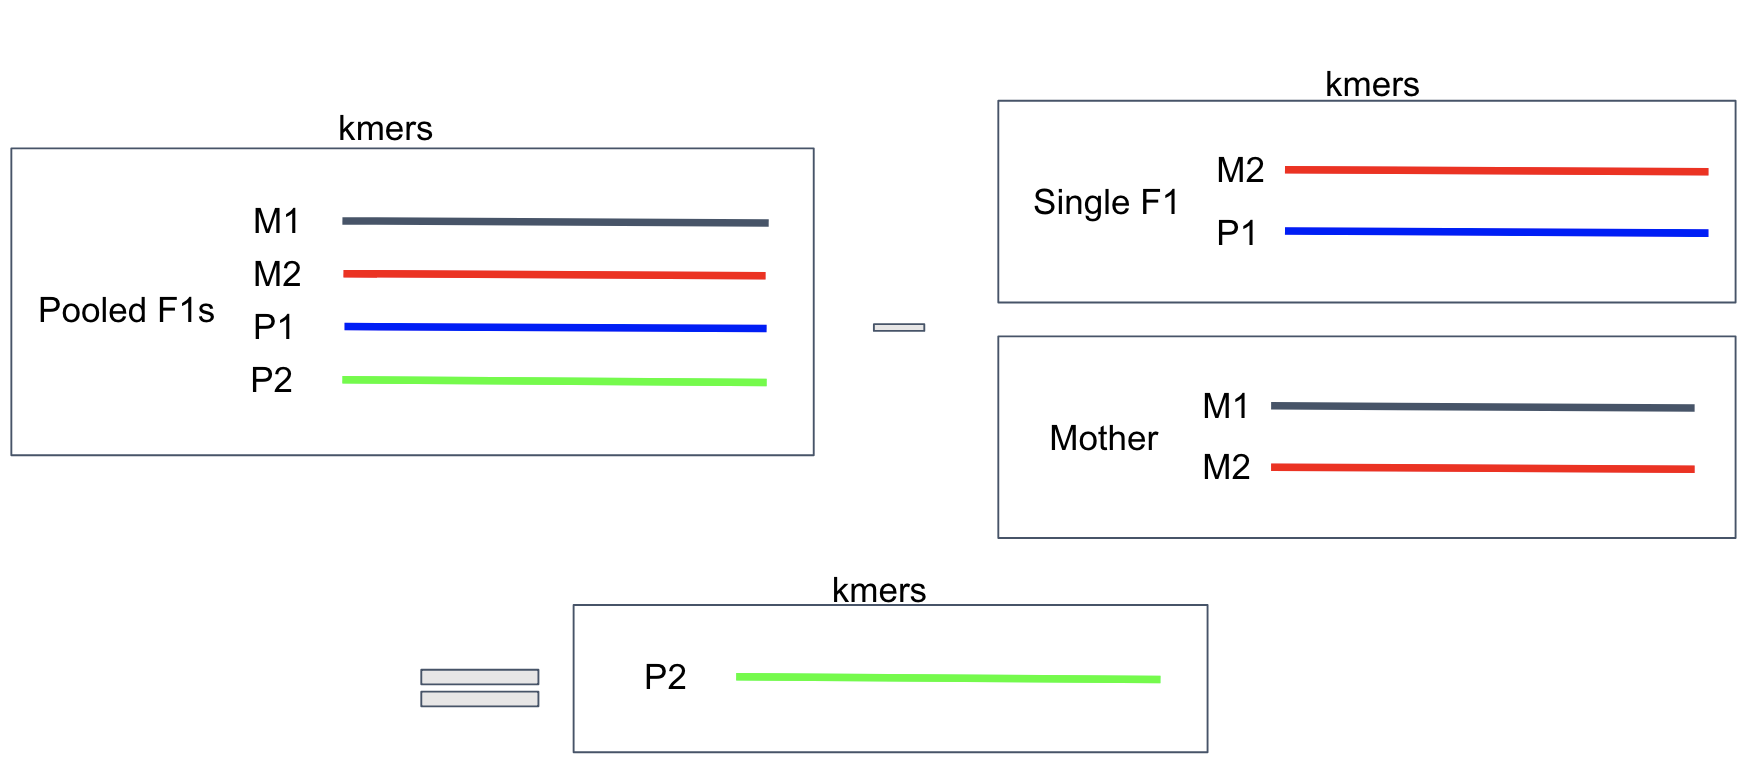
\includegraphics[width=\textwidth]{pseudotrio.png}
\end{centering}
\end{figure}

As shown in \ref{figure:pseudotrio} we can obtain distinguishing kmers for the P1 haplotype by set subtraction of kmers in the maternal and single F1 sample 
from the those in the pooled samples. In a similar way we can subtract kmers in the maternal sample from the single F1 sample to get probabilistic distinguishing 
kmers from the P2 haplotype. We say probabilistic distinguishing kmers because these kmers could also occur on the P1 haplotype as well. And in the same way 
we can get probabilistic distinguishing kmers for the M1 haplotype by subtracting kmers in the single F1 sample from those in the maternal sample. And finally we can obtain 
probabilistic distinguishing kmers for the M2 haplotype will be obtained by selecting kmers which are shared between the maternal and single F1 sample and occur at 
haploid counts in both samples. Once we have these distinguishing kmers we can use them to separate long reads by haplotype for libraries created from any of these samples. 
We have created software for collecting these distinguishing kmers \cite{distinguishing_kmers} which uses counting bloom filters to minimize memory usage 
and a mod based system allowing distribution of jobs to many worker nodes. And we also have software for binning long reads based on those 
distinguishing kmers \cite{long_read_binner}.


\section{Phasstools: phasing and assembly tools}
\subsection{Heterozygous kmer pairs and detection}
First we tackle the subject of identifying heterozygous variants in a reference-free manner. We will do this using a kmer approach, as many reference-free methods do. 
Many people have focused on identifying kmers which occur at roughly half counts in short read data \cite{KAT} and various software exists to count kmers \cite{jellyfish} 
and to model the mixture of expected distributions (errors, haploid, diploid, duplication kmers) \cite{genomescope}. Identifying heterozygous kmers in this way 
suffers from multiple problems from the perspective of de novo phasing. 1. Many of these identified as half counts will be either randomly high count error kmers or randomly low count 
homozygous kmers. 2. You end up with $K-1$ overlapping kmers for a given variant which is needlessly redundant information which will both slow down any phasing algorithm and 
likely break key independence assumptions. And 3. while you have heterozygous kmers, you don't know which kmers are alternative alleles of each other. 
We propose finding pairs of kmers which vary only in the center position which are also both roughly at half counts. These heterozgyous SNP kmers 
will be much more robust and have the benefit of knowing that one is the alternative allele of the other.
We have software for this purpose \cite{het_kmers} which uses counting bloom filters to minimize memory usage and a mod based method to 
distribute the work to many worker nodes.

\subsection{Phasing consistency}

\subsection{Data types and uses}


\subsection{Phasst phase: Reference or assembly based phasing}
\subsubsection{Sparse \textit{Bernoulli} mixture model clustering}
\subsubsection{Polyploid phasing}
\subsubsection{Phasing consistency genotype correction}
\subsection{Phasst a: phased assembly}
\subsubsection{Phasing consistent heterozygous kmer recruitment}
\subsubsection{Haplotype and chromosome read binning}
\subsubsection{Haploid chromosome assemly}
\subsection{Phasst scaff: phasing aware assembly scaffolding}
\subsubsection{Chromosome binning}
\subsubsection{Ordering and Orienting}


%\section{De novo haplotype phasing}
In order to separate long reads by haplotype for a single individual, we must develop an algorithm for de novo haplotype phasing. In reference based systems, haplotype 
phasing begins by mapping reads to the reference and calling variants from the reference. Then physical linkage information of two heterozygous variants occurring 
on data known to be generated from a single haplotype is used to determine which alleles come from which of the sister chromosomes across 
either some region (denoted as a phase block) or 
across whole chromosomes \cite{10xlinked} \cite{whatshap} \cite{hapcut2} \cite{hapchat}. At each heterozygous variant locus, one allele can arbitrarily be denoted as 0 and 
the second allele denoted 1. Then without loss of generality we choose to represent the series of alleles located on whichever chromosome has the 0 allele of the first variant in 
a phase block. So now the problem can be seen as determining the binary sequence of which alleles are on that same chromosome that are most consistent 
with the linkage data we have. To do this, each of these methods uses different search strategies (beam search, dynamic programming, graph based heuristic search) to find the 
configuration that maximizes the probability of the data under some error model. These algorithms are also aided by the knowledge of which variants are close to each other (and 
thus are most likely to contain linkage information) on the genome. It is common to proceed in a directed manner, determining the optimal solution for variants $[0..n-1]$ before 
determining the phase of variant $n$. So for de novo haplotype phasing we will need to 1. identify heterozygous alleles 2. determine an ordering of those alleles and 3. create a 
search strategy to maximize a probabilistic model of the data. 



\subsubsection{Diploid assembly validation}

While certain tools for assembly validation are available \cite{KAT} \cite{busco}, the validation of diploid assemblies is a difficult problem still in its infancy. 
These heterozygous kmers are also useful for validating diploid assemblies because you expect to see one of the heterozygous kmer pairs in the primary assembly 
and the other one in the secondary haplotigs. If, for instance, you find both versions of a heterozygous kmer pair in the primary assembly, this could either represent residual 
heterozygosity in the primary assembly which should be removed, or perhaps the kmers came from paralogous regions and both kmers had lower than homozygous counts 
due to random sampling error. Another error type that exists is lacking either of the kmer pair in the primary which could represent low base level accuracy, over collapse of near repeat regions, or some other type of error. Other cases exist which may have their own interpretations. We have developed software for this analysis which is now in use by the Sanger 
assembly curation team \cite{haplovalidate}.

%\subsection{De novo phasing algorithm strategy}
The next step for de novo phasing is determining a rough ordering of heterozygous SNPs. If we view the heterozygous kmers as nodes in a graph and edges between 
nodes as linkage information of long reads or other long genetic distance linkage information with weights as the number of those links, we could view our problem as a 
graph based traveling salesman problem in which we want to find the maximum scoring traversal of nodes in which each node is only visited once. While the traveling salesman 
problem is known to be an NP-hard problem, greedy approximation algorithms exist with fast implementations \cite{randomwalkTSP}, and we don't need the true optimal ordering. 
We just need an ordering such that heterozygous SNPs near one another in the ordering are likely to share linkage information in our data.

Once we have a pseudo ordering of heterozygous SNP kmers, we could proceed in many different ways including methods which already exist \cite{10xlinked}. 
Or we could approach the problem from a novel angle with some benefits. We propose to solve the haplotype phasing search problem with mixture model clustering. In this case, 
each cluster center would be a vector of length $n$ where $n$ is the number of heterozgyous kmers in some chunk which we believe should share linkage and the values in that 
vector would represent the allele fraction on that haplotype of one of the alleles chosen arbitrarily. When optimized, these values would tend toward 0 and 1 assuming the data 
supports a diploid structure.  Similar to our single cell genotype clustering algorithm, we marginalize each read 
across the possible haplotypes. Then the negative log likelihood should be differentiable and susceptible to numerical optimization techniques. This method has several potential 
advantages over current approximation search algorithms. One is that is is trivially extendable to polyploid genomes. In the polyploid case, the only thing that changes is that there are $P = ploidy$ cluster centers instead of just two. Another benefit is that it can handle cases in which one of the variants chosen is not actually heterozygous but is homozygous for one 
of the alleles. Including these cases can dramatically slow down current algorithms, but is beneficial in error correcting variant calls \cite{10xpatent}. This algorithm could also be used 
in reference based systems.

\section{Discussion}

